\documentclass[10pt]{beamer}

\usepackage{graphicx}
\usepackage{amsmath}
\usepackage{bm}
\usepackage{array}
\usepackage{adjustbox}

% New Commands
\newcommand*{\Scale}[2][4]{\scalebox{#1}{$#2$}}%
\newcommand{\quart}[4]{\begin{picture}(80,6)
    {\color{black}\put(#3,3){\circle*{2.5}}\put(#1,3){\line(1,0){#2}}}\end{picture}
}


\usetheme{default}
\usecolortheme{dove}
\title{Evolutionary Multi-Objective Optimization:}
\subtitle{\Large A Parallel Computing Approach}
\author{Rahul Krishna \and George Mathew}
% - Give the names in the same order as the appear in the paper.
% - Use the \inst{?} command only if the authors have different
%   affiliation.

\institute[NC State University] % (optional, but mostly needed)
{
  \inst{}%
  Department of Computer Science\\
  North Carolina State University}
% - Use the \inst command only if there are several affiliations.
% - Keep it simple, no one is interested in your street address.

\date{\today}
% - Either use conference name or its abbreviation.
% - Not really informative to the audience, more for people (including
%   yourself) who are reading the slides online

\subject{CSC 591: Experimental Algorithms, Fall 2015}
% This is only inserted into the PDF information catalog. Can be left
% out. 

% If you have a file called "university-logo-filename.xxx", where xxx
% is a graphic format that can be processed by latex or pdflatex,
% resp., then you can add a logo as follows:

% \pgfdeclareimage[height=1cm]{university-logo}{figures/CSClogo}
% \logo{\pgfuseimage{university-logo}}
\logo{
\includegraphics[height=1cm]{figures/CSClogo}\vspace{260pt}}
% \logo{
\includegraphics[width=0.99cm]{figures/NCRedRibbon}}

% Delete this, if you do not want the table of contents to pop up at
% the beginning of each subsection:
\AtBeginSubsection[]
{
  \begin{frame}<beamer>{Outline}
  \scriptsize{
    \tableofcontents[currentsection,currentsubsection]}
  \end{frame}
}

% Let's get started
\begin{document}

\begin{frame}
  \titlepage
\end{frame}

\begin{frame}{Outline}
  \scriptsize{\tableofcontents}
  % You might wish to add the option [pausesections]
\end{frame}

% Section and subsections will appear in the presentation overview
% and table of contents.
\section{Background}

\subsection{$\rightarrow$ Multi-Objective Problem}
\begin{frame}{Multi-Objective Problem}
  \begin{minipage}{0.45\linewidth}
  \footnotesize{
  \begin{itemize}
  \item<2-> \textbf{Pareto Frontier} State of solutions which are equally good.
  \item<3-> \textbf{Pareto Point} A point that lies on the Pareto frontier.
  \item<4-> \textbf{Feasible Point} A satisfiable solution for the problem but not necessarily the optimum one.
  \item<5-> \textbf{Infeasible Point} A solution outside the Pareto frontier
  \item<6-> \textbf{Utopia Point} The ideal theoretical solution we would love to reach but practically its not possible
  \end{itemize}}
  \end{minipage}~~\begin{minipage}{0.40\linewidth}
  \begin{figure}
  \centering
  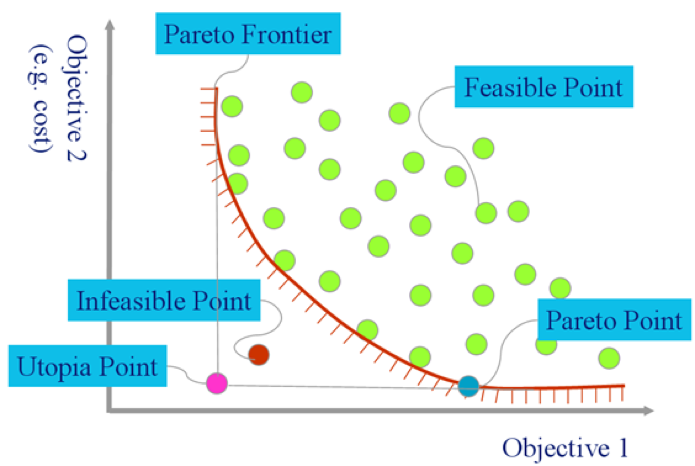
\includegraphics[width=\linewidth]{figures/Picture1}
  \caption{Sample Pareto Frontier}
  \label{fig:my_label}
  \end{figure}
  \end{minipage}
\end{frame}

\section{Models}
\subsection{$\rightarrow$ DTLZ2}
\begin{frame}{DTLZ-2}
  \begin{minipage}{0.60\linewidth}
  \footnotesize{
  \begin{itemize}
  \item \textbf{Decisions} DTLZ-2 has 30 decisions where each decision ranges between 0 and 1.
  \[\Scale[0.8]{0 \leq {x}_{i} \leq 1 \ \ \ \ where \ \  i = 1,2 ,3 .... 30}\]
  \item \textbf{Objectives} A point that lies on the Pareto frontier.
  \[\Scale[0.75]{{f}_{1}(x) = (1+g({x}_{M}))\cos({x}_{1} \pi/2)....\cos({x}_{M-1} \pi/2)}\]
  \[\Scale[0.75]{{f}_{2}(x) = (1+g({x}_{M}))\cos({x}_{1} \pi/2)....\cos({x}_{M-1} \pi/2)}\]
  \[\Scale[0.75]{{f}_{3}(x) = (1+g({x}_{M}))\sin({x}_{1} \pi/2)}\]
  \[\Scale[0.75]{where \ \ \ \ g({x}_{M}) = \sum_{x \in {x}_{M}} (x_i - 0.5)^2} \]
  \item \textbf{Optimal Solution:} Ideal Decisions are $x_i=0.5$ where $i=1,2,3...30$
  \\
  Ideal objectives should satisfy the equation $\sum_{m=1}^{3} f_m^2 = 1$
  \end{itemize}}
  \end{minipage}
  \noindent
  \begin{minipage}{0.35\linewidth}
  \begin{figure}
  \centering
  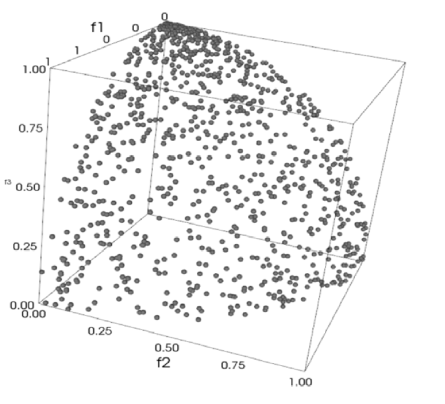
\includegraphics[width=\linewidth]{figures/dtlz2pf}
  \caption{Pareto Frontier}
  \label{fig:de_pf}
  \end{figure}
  \end{minipage}
\end{frame}
  
\subsection{$\rightarrow$ XOMO}
\begin{frame}{XOMO}
\begin{itemize}
\item<1-> Monte Carlo Simulator modelling NASA's space program software.
\item<2-> 23 decisions - lines of code, storage, cyclometric complexity etc.
\item<3-> 4 objectives all minimized
    \begin{itemize}
    \item<3-> Total Developer \textbf{Effort}.
    \item<3-> \textbf{Months} to complete project.
    \item<3-> Total \textbf{Defects} in project.
    \item<3-> \textbf{Risk} involved in project.
    \end{itemize}
\end{itemize}
\end{frame}
\subsection{$\rightarrow$ POM3}
\begin{frame}{POM3}
\begin{itemize}
\item<1-> Implements Boehm \& Turner model of agile programming 
\item<2-> Teams select tasks as they appear in the scrum backlog.
\item<3-> 9 decisions like size of project, project plan, team size etc.
\item<4-> The model contains 4 objectives
    \begin{itemize}
    \item<4-> Minimize \textbf{Cost}.
    \item<4-> Maximize \textbf{Utility}.
    \item<4-> Maximize \textbf{Completion Percentage}.
    \item<4-> Minimize \textbf{Idle Time} for Developers.
    \end{itemize}
\end{itemize}
\end{frame}

\section{Algorithms}
\subsection{$\rightarrow$ Evolutionary Algorithm}
\begin{frame}{Evolutionary Algorithm}
    \begin{figure}
    \centering
    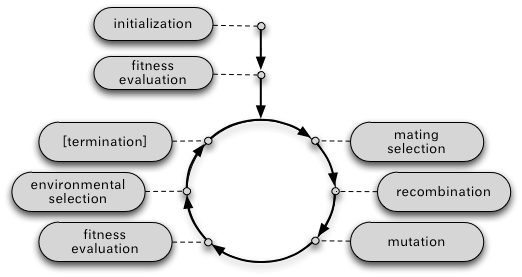
\includegraphics[width=\linewidth]{figures/evo_algo}
    \label{fig:evo_algo}
    \end{figure}
\end{frame}
\subsection{$\rightarrow$ Differential Evolution}
\begin{frame}{Differential Evolution(DE)}
    \begin{itemize}
    \item<1-> Stochastic evolutionary optimization technique.
    \item<2-> Iteratively approximates the shape of the Pareto Frontier
    \item<3-> Advantages:
    \begin{itemize}
        \item<3-> Simple \& Computationally Inexpensive.
        \item<3-> High dimensional problems can be handled easily.
        \item<3-> Solutions are very stable.
    \end{itemize}
    \end{itemize}
\end{frame}
\begin{frame}{DE - Algorithm}
    \begin{figure}
    \centering
    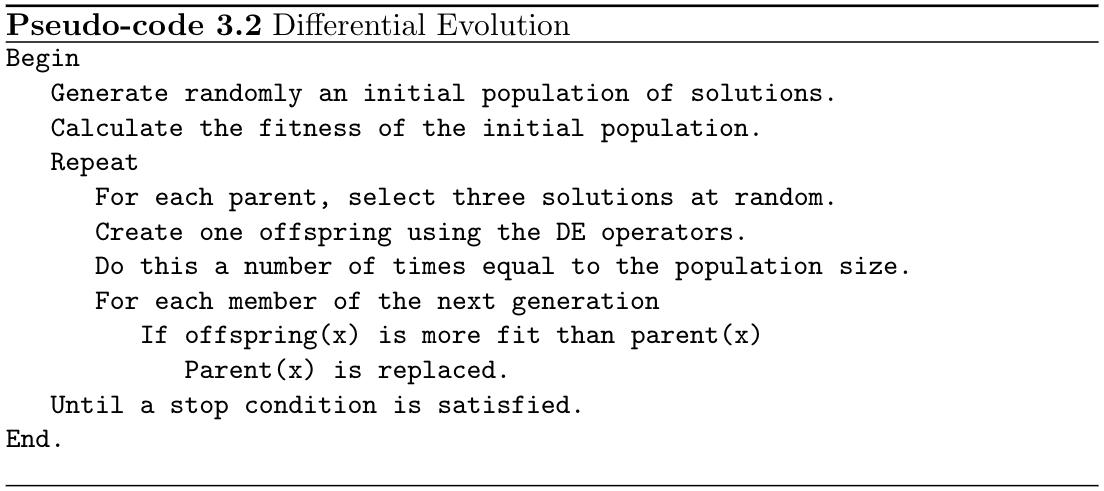
\includegraphics[width=\linewidth]{figures/DE_pseudocode}
    \label{fig:de_pseudocode}
    \end{figure}
\end{frame}
\subsection{$\rightarrow$ GALE: Geometric Active Learner}
\begin{frame}{Geometric Active LEarner (GALE)}
    \begin{itemize}
    \item<1-> Near linear time Multi-Objective Evolutionary Algorithm.
    \item<2-> Builds piecewise approximation to the best solutions of the pareto frontier.
    \item<3-> Based on WHERE which is a recursive clustering technique based on Dimensionality Reduction.
    \item<4-> Advantages:
    \begin{itemize}
        \item<4-> Less Number of Computations.
        \item<4-> Adept at handling problems that are \textbf{non-differentiable}, \textbf{non-liner}, \textbf{multi-dimensional} or \textbf{multi-constraint}.
        \item<4-> Concise representation of problem space.
    \end{itemize}
    \end{itemize}
\end{frame}
\begin{frame}{GALE - Algorithm}
    \begin{itemize}
    \item<1-> Cluster data based on WHERE
        \begin{columns}[t]
            \begin{column}{0.3\linewidth}
                \begin{figure}
                    \centering
                    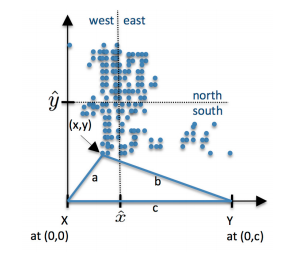
\includegraphics[scale=0.4]{figures/where}
                    \label{fig:where}
                \end{figure}
                %\adjincludegraphics[scale=0.4,valign=t]{figures/where}
            \end{column}
            \begin{column}{0.7\linewidth}
            \begin{itemize}
                \item<2-> Pick point \textbf{\textit{X}} from the cluster. Then pick point \textbf{\textit{East}} furthest from \textbf{\textit{X}} and point \textbf{\textit{West}} furthest from \textbf{\textit{East}}. Let \textbf{\textit{c}} be the distance between \textbf{\textit{East}} and \textbf{\textit{West}}.
                \item<3-> For every other point in the cluster, compute \textbf{\textit{a}} and \textbf{\textit{b}} which represents distance of the point from \textbf{\textit{East}} and \textbf{\textit{West}} respectively.
                \item<4-> Compute the projection \textbf{\textit{x}} as \(\bm{x}=(\bm{a}^2+\bm{c}^2-\bm{b}^2)/2\bm{c}\)
            \end{itemize}
            \end{column}
        \end{columns}
    \item<5-> Select the best point from the non-dominated cluster and mutate towards it and store the best points.
    \item<6-> Repeat for \textbf{\textit{n}} generations.
    \end{itemize}
\end{frame}
\section{Parallelization Strategies}
\subsection{$\rightarrow$ The Island Model}
\begin{frame}{Island Model}
    \begin{minipage}{0.48\linewidth}
        \begin{itemize}
            \item<1-> Divide the initial population(\textbf{\textit{N}}) into sub-populations of equal size(\textbf{\textit{n}}) among \textbf{\textit{k}} processors.
            \[ n = {N \over k}\]
            \item<2-> Evolve each sub-population independently.
            \item<3-> Aggregate the final population of each processor after the total number of generations.
        \end{itemize}
    \end{minipage}
    \begin{minipage}{0.5\linewidth}
        \begin{figure}
            \centering
            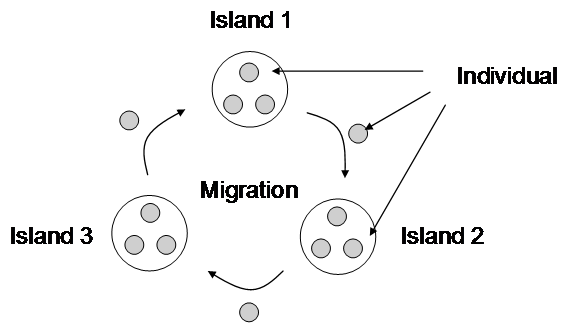
\includegraphics[scale=0.25]{figures/island}
            \label{fig:island}
        \end{figure}
    \end{minipage}
\end{frame}
\subsection{$\rightarrow$ Master-Slave Model}
\begin{frame}{Master-Slave Model}
    \begin{minipage}{0.48\linewidth}
        \begin{itemize}
            \item<1-> Master selects a population for each free slave in each generation.
            \item<2-> Slave evaluates the fitness and computes the best solution(s) for each population set.
            \item<3-> Slave performs mutation on each population subset and sends it to master for next generation.
        \end{itemize}
    \end{minipage}
    \begin{minipage}{0.5\linewidth}
        \begin{figure}
            \centering
            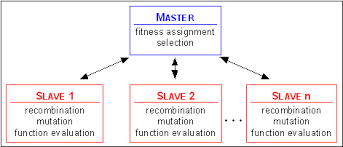
\includegraphics[scale=0.5]{figures/master-slave}
            \label{fig:master-slave}
        \end{figure}
    \end{minipage}
\end{frame}

\section{Evaluation Metrics}
\subsection{$\rightarrow$ Evaluation}
\begin{frame}{Evaluation}
    \begin{itemize}
    \item<1-> \textbf{Runtime:} Time taken to run the algorithm. This can be measured using a profiler.
    \item<2-> \textbf{Speed-Up:} Serialized Runtime version of the algorithm over the Parallelized version of it.
    \item<3-> \textbf{Solution Quality:}
    \begin{columns}[t]
    \begin{column}{0.6\linewidth}
    \begin{itemize}
    \item<4-> \textbf{Convergence:}
        \begin{itemize}
            \item<4-> Accuracy of the obtained solutions.
            \item<4-> Represents the HyperVolume between the obtained solutions and Pareto Frontier
        \end{itemize}
    \item<5-> \textbf{Diversity:}
        \begin{itemize}
            \item<5-> Spread of the proposed solutions.
            \item<5-> Ideally the solutions should be well distributed across the Pareto Frontier
        \end{itemize}
    \end{itemize}
    \end{column}
    \begin{column}{0.4\linewidth}
        \begin{figure}
            \centering
            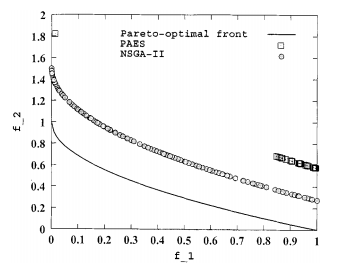
\includegraphics[scale=0.35]{figures/conv_div}
            \label{fig:conv_div}
        \end{figure}
    \end{column}
    \end{columns}
    \end{itemize}
\end{frame}

\subsection{$\rightarrow$ Measures}
\begin{frame}{Measures}
\begin{columns}[t]
    \begin{column}{0.5\linewidth}
    \textbf{Convergence:}
    \begin{figure}
        \centering
        \includegraphics[scale=0.35]{figures/convergence}
        \label{fig:convergence}
    \end{figure}
    \footnotesize{\begin{itemize}
    \item Find a set of H optimal solutions.
    \item For each solution, compute the minimum eucledian distance from each of the solutions to a point on the Pareto Frontier.
    \item The average of these distances represent convergence.
    \end{itemize}}
    \end{column}
    \begin{column}{0.5\linewidth}
    \textbf{Diversity:}
    \begin{figure}
        \centering
        \includegraphics[scale=0.35]{figures/diversity}
        \label{fig:diversity}
    \end{figure}
    \footnotesize{\begin{itemize}
    \item $d_i$ is the distance between consecutive solutions.
    \item $\bar{d}$ is the mean of $d_i$ 
    \item $d_f$ \& $d_l$ are distance between extreme and boundary solutions.
    \[\Delta = {{d_f + d_l + \sum_{i=1}^{N-1}|d_i-\bar{d}|}\over{d_f + d_l + (N-1)\bar{d}}}\]
    \end{itemize}}
    \end{column}
\end{columns}
\end{frame}

\section{Experimental Setup}
\begin{frame}{Experimental Setup}
    \begin{itemize}
    \item<1-> \textbf{Python}
        \begin{itemize}
        \item Support for scientific computation: numpy, scipy, etc.
        \item Quick prototyping and benchmarking.
        \end{itemize}
    \item<2-> \textbf{Open-MPI}
        \begin{itemize}
        \item Open Source Message Passing Interface with Python wrapper.
        \item The Open MPI Project is actively developed and maintained by a consortium of academic, research, and industry partners.
        \end{itemize}
    \item<3-> \textbf{Multi-Processing}
        \begin{itemize}
        \item Offers local and remote concurrency.
        \item Overrides python Global Interpreter Lock.
        \end{itemize}
    \item<4-> \textbf{HPC}
        \begin{itemize}
        \item The henry2 shared memory linux cluster at NCSU.
        \item Up to 16 shared memory processor cores and up to 128GB of memory accessible through a dedicated queue.
        \end{itemize}
    \end{itemize}
\end{frame}

\section{Results}
\subsection{$\rightarrow$ Island Model}
\begin{frame}{DTLZ-2(Island Model)}
    \begin{figure}
		\centering
        \includegraphics[scale=0.25]{figures/island/dtlz2/convergence}
        \caption{Convergence of serial \& parallel DE \& GALE}
        \label{fig:DTLZ2_convergence}
	\end{figure}
	\pause
	\begin{figure}
		\centering
        \includegraphics[scale=0.25]{figures/island/dtlz2/diversity}
        \caption{Diversity of serial \& parallel DE \& GALE}
        \label{fig:DTLZ2_diversity}
	\end{figure}
\end{frame}
\begin{frame}{DTLZ-2(Island Model)}
    \begin{columns}[t]
        \begin{column}{0.5\linewidth}
        \textbf{Runtimes:}
        \begin{figure}
            \centering
            \includegraphics[scale=0.27]{figures/island/dtlz2/DE_runtimes}
            \label{fig:DTLZ2_DE_runtimes}
        \end{figure}
        \begin{figure}
            \centering
            \includegraphics[scale=0.27]{figures/island/dtlz2/GALE_runtimes}
            \label{fig:DTLZ2_GALE_runtimes}
        \end{figure}
        \end{column}
        \begin{column}{0.5\linewidth}
        \textbf{Speed Ups:}
        \begin{figure}
            \centering
            \includegraphics[scale=0.36]{figures/island/dtlz2/speedups}
            \label{fig:DTLZ2_speedups}
        \end{figure}
        \end{column}
    \end{columns}
\end{frame}
\begin{frame}{POM3(Island Model)}
    \begin{columns}[t]
        \begin{column}{0.5\linewidth}
        \textbf{Runtimes:}
        \begin{figure}
            \centering
            \includegraphics[scale=0.36]{figures/island/pom3/runtimes}
            \label{fig:POM3_runtimes}
        \end{figure}
        \end{column}
        \begin{column}{0.5\linewidth}
        \textbf{Speed Ups:}
        \begin{figure}
            \centering
            \includegraphics[scale=0.36]{figures/island/pom3/speedups}
            \label{fig:POM3_speedups}
        \end{figure}
        \end{column}
    \end{columns}
\end{frame}
\begin{frame}{XOMO(Island Model)}
    \begin{columns}[t]
        \begin{column}{0.5\linewidth}
        \textbf{Runtimes:}
        \begin{figure}
            \centering
            \includegraphics[scale=0.27]{figures/island/xomo/DE_runtimes}
            \label{fig:XOMO_DE_runtimes}
        \end{figure}
        \begin{figure}
            \centering
            \includegraphics[scale=0.27]{figures/island/xomo/GALE_runtimes}
            \label{fig:XOMO_GALE_runtimes}
        \end{figure}
        \end{column}
        \begin{column}{0.5\linewidth}
        \textbf{Speed Ups:}
        \begin{figure}
            \centering
            \includegraphics[scale=0.36]{figures/island/xomo/speedups}
            \label{fig:XOMO_speedups}
        \end{figure}
        \end{column}
    \end{columns}
\end{frame}

\subsection{$\rightarrow$ Master-Slave Model}
\begin{frame}{DTLZ-2(Master-Slave Model)}
    \begin{columns}[t]
        \begin{column}{0.5\linewidth}
        \textbf{Runtimes:}
        \begin{figure}
            \centering
            \includegraphics[scale=0.27]{figures/master-slave/dtlz2/DE_runtimes}
            \label{fig:DTLZ2_MS_DE_runtimes}
        \end{figure}
        \begin{figure}
            \centering
            \includegraphics[scale=0.27]{figures/master-slave/dtlz2/GALE_runtimes}
            \label{fig:DTLZ2_MS_GALE_runtimes}
        \end{figure}
        \end{column}
        \begin{column}{0.5\linewidth}
        \textbf{Speed Ups:}
        \begin{figure}
            \centering
            \includegraphics[scale=0.36]{figures/master-slave/dtlz2/speedups}
            \label{fig:DTLZ2_MS_speedups}
        \end{figure}
        \end{column}
    \end{columns}
\end{frame}
\begin{frame}{POM3(Master-Slave Model)}
    \begin{columns}[t]
        \begin{column}{0.5\linewidth}
        \textbf{Runtimes:}
        \begin{figure}
            \centering
            \includegraphics[scale=0.36]{figures/master-slave/pom3/runtimes}
            \label{fig:POM3_MS_runtimes}
        \end{figure}
        \end{column}
        \begin{column}{0.5\linewidth}
        \textbf{Speed Ups:}
        \begin{figure}
            \centering
            \includegraphics[scale=0.36]{figures/master-slave/pom3/speedups}
            \label{fig:POM3_MS_speedups}
        \end{figure}
        \end{column}
    \end{columns}
\end{frame}
\begin{frame}{XOMO(Master-Slave Model)}
    \begin{columns}[t]
        \begin{column}{0.5\linewidth}
        \textbf{Runtimes:}
        \begin{figure}
            \centering
            \includegraphics[scale=0.36]{figures/master-slave/xomo/runtimes}
            \label{fig:XOMO_MS_DE_runtimes}
        \end{figure}
        \end{column}
        \begin{column}{0.5\linewidth}
        \textbf{Speed Ups:}
        \begin{figure}
            \centering
            \includegraphics[scale=0.36]{figures/master-slave/xomo/speedups}
            \label{fig:XOMO_MS_speedups}
        \end{figure}
        \end{column}
    \end{columns}
\end{frame}

\section{Future Work}
\subsection{$\rightarrow$ Feature Models}
\begin{frame}{Feature Model}
\begin{itemize}
\item<1-> A \textbf{feature model} is a compact representation of all the products of the Software Product Line in terms of "features". Feature models are visually represented by means of feature diagrams.
\item<2-> Parent and Child features are categorized as
    \begin{itemize}
        \item<2-> \textbf{Mandatory} – child feature is required.
        \item<2-> \textbf{Optional} – child feature is optional.
        \item<2-> \textbf{Or} – at least one of the sub-features must be selected.
        \item<2-> \textbf{Alternative} – one of the sub-features must be selected.
    \end{itemize}
\item<3-> For our experiment we use the Emergency Response(ERS) feature model, which has \textbf{35 decisions} and \textbf{3 objectives}. 
\end{itemize}

\end{frame}



\subsection{$\rightarrow$ Results: Feature Models}
\begin{frame}{Emergency Response(Island Model)}
    \begin{columns}[t]
        \begin{column}{0.5\linewidth}
        \textbf{Runtimes:}
        \begin{figure}
            \centering
            \includegraphics[scale=0.36]{figures/island/ers/runtimes}
            \label{fig:ERS_runtimes}
        \end{figure}
        \end{column}
        \begin{column}{0.5\linewidth}
        \textbf{Speed Ups:}
        \begin{figure}
            \centering
            \includegraphics[scale=0.36]{figures/island/ers/speedups}
            \label{fig:ERS_speedups}
        \end{figure}
        \end{column}
    \end{columns}
\end{frame}


\subsection{$\rightarrow$ Other Extensions:}
\begin{frame}{Other Extensions:}
    \begin{itemize}
    \item<1-> Mutation strategies for real world problems which are heavily constrained.
    \item<2-> Extending these parallelization strategies for other Evolutionary algorithms like NSGA2, SPEA, IBEA etc
    \item<3-> Strategies for efficiently dividing the feature space for parallelization.
    \end{itemize}

\end{frame}

\section*{Summary}
\subsection*{$\rightarrow$ In Conclusion..}
\begin{frame}{In Conclusion..}
\begin{itemize}
\item<1-> Parallelization is effective for Multi Objective Evolutionary Algorithms.
\item<2-> Differential Evolution is preferred for Mathematical Problems.
\item<3-> GALE is preferred for Real-World Problems where model evaluation is expensive.
\end{itemize}

\end{frame}

\end{document}


